% ============================================================================
% AgentClinic MTP — Comprehensive Thesis Progress Report
% IIT Kharagpur | April 2026
% Dikshant Sharma
% ============================================================================
\documentclass[12pt, a4paper]{article}

% --- Packages ---
\usepackage[utf8]{inputenc}
\usepackage[T1]{fontenc}
\usepackage[margin=2.5cm]{geometry}
\usepackage{graphicx}
\usepackage{booktabs}
\usepackage{array}
\usepackage{longtable}
\usepackage{xcolor}
\usepackage{listings}
\usepackage{hyperref}
\usepackage{amsmath}
\usepackage{amssymb}
\usepackage{enumitem}
\usepackage{fancyhdr}
\usepackage{titlesec}
\usepackage{tcolorbox}
\usepackage{mdframed}
\usepackage{float}
\usepackage{caption}
\usepackage{subcaption}
\usepackage{multirow}
\usepackage{tikz}
\usetikzlibrary{arrows.meta, positioning, fit, shapes}

% --- Hyperref Setup ---
\hypersetup{
    colorlinks=true,
    linkcolor=blue!70!black,
    citecolor=green!50!black,
    urlcolor=cyan!70!black
}

% --- Header/Footer ---
\pagestyle{fancy}
\fancyhf{}
\fancyhead[L]{\textbf{AgentClinic v2.1 — MTP Progress Report}}
\fancyhead[R]{Dikshant Sharma | IIT Kharagpur}
\fancyfoot[C]{\thepage}

% --- Color Definitions ---
\definecolor{codebg}{RGB}{245, 245, 250}
\definecolor{successpink}{RGB}{0, 150, 80}
\definecolor{warnred}{RGB}{180, 30, 30}
\definecolor{iitblue}{RGB}{0, 64, 128}
\definecolor{noteblue}{RGB}{210, 230, 255}

% --- Code listing Style ---
\lstdefinestyle{bashstyle}{
    backgroundcolor=\color{codebg},
    basicstyle=\ttfamily\footnotesize,
    breaklines=true,
    frame=single,
    rulecolor=\color{gray!40},
    numbers=left,
    numberstyle=\tiny\color{gray},
    keywordstyle=\color{blue},
    commentstyle=\color{green!60!black},
    language=bash
}
\lstdefinestyle{pystyle}{
    backgroundcolor=\color{codebg},
    basicstyle=\ttfamily\footnotesize,
    breaklines=true,
    frame=single,
    rulecolor=\color{gray!40},
    numbers=left,
    numberstyle=\tiny\color{gray},
    keywordstyle=\color{blue!80!black},
    stringstyle=\color{orange!80!black},
    commentstyle=\color{green!60!black},
    language=Python
}

% --- Section Title Styling ---
\titleformat{\section}[block]{\large\bfseries\color{iitblue}}{\thesection.}{0.5em}{}[\titlerule]
\titleformat{\subsection}[block]{\normalsize\bfseries\color{iitblue!80!black}}{\thesubsection.}{0.5em}{}

% ============================================================================
\begin{document}
% ============================================================================

% --- Title Page ---
\begin{titlepage}
    \centering
    \vspace*{2cm}
    {\Huge\bfseries\color{iitblue} AgentClinic v2.1\\[0.4em]
    \large A Multi-Agent LLM Framework for\\Clinical Decision-Making\\[0.3em]}
    {\Large\color{gray} M.Tech Thesis Progress Report}
    \vspace{1.5cm}
    \hrule height 1pt
    \vspace{0.5cm}

    \begin{minipage}{0.48\textwidth}
        \textbf{Author:} Dikshant Sharma\\
        \textbf{Programme:} M.Tech, IIT Kharagpur\\
        \textbf{GitHub:} \href{https://github.com/DikshantSh/AgentClinic_MTP}{DikshantSh/AgentClinic\_MTP}
    \end{minipage}
    \hfill
    \begin{minipage}{0.48\textwidth}
        \textbf{Date:} April 2026\\
        \textbf{Status:} E1 Complete, E2 In Progress\\
        \textbf{Hardware:} NVIDIA H100 NVL (95.8 GB)
    \end{minipage}

    \vspace{0.5cm}
    \hrule height 1pt
    \vspace{1.5cm}

    \begin{tcolorbox}[colback=noteblue, colframe=iitblue!60, title=\textbf{Purpose of This Document}]
        This report serves as a \textbf{comprehensive reference document} for:
        \begin{enumerate}
            \item The thesis author — as a running record of design decisions, results, and blockers.
            \item Future AI agents — to \textbf{resume work} with full context without re-reading all source code.
            \item The thesis committee — as a technical summary of methodology and preliminary results.
        \end{enumerate}
    \end{tcolorbox}

    \vfill
    \tableofcontents
\end{titlepage}

\newpage

% ============================================================================
\section{Project Overview}
% ============================================================================

\subsection{Research Objective}

The central thesis question is:

\begin{mdframed}[backgroundcolor=noteblue, linecolor=iitblue, linewidth=1.5pt]
\textit{"Do medically fine-tuned LLMs outperform general-purpose LLMs as physician agents in a multi-agent clinical diagnostic simulation? And how do cognitive biases (recency, confirmation) affect diagnostic accuracy and process quality?"}
\end{mdframed}

\vspace{0.5em}
The study operationalises this through a multi-agent simulation (\textbf{AgentClinic v2.1}) where distinct LLM ``roles'' (Doctor, Patient, Measurement Reader, Moderator) interact through structured clinical dialogue to reach a diagnosis, evaluated both on \textbf{outcome accuracy} (correct diagnosis vs. MedQA ground truth) and \textbf{process quality} (diagnostic stability, test rationality, information efficiency).

\subsection{Starting Point (Phase 1 — Legacy System)}

The project began with \texttt{agentclinic\_ninthcache.py}, a \textbf{legacy while-loop} based system which had the following major limitations:
\begin{itemize}
    \item No deterministic state management (agent turns not guaranteed to be ordered).
    \item Cognitive biases were implemented \textit{in-prompt only}, with no separate tracking.
    \item Process-oriented metrics (diagnostic stability, test rationality) were computed \textit{post-hoc} in a separate script (\texttt{evaluation\_updated.py}), not inline.
    \item Only API-based models (OpenAI, Anthropic, Replicate) were supported — no local model inference.
    \item No heterogeneous architecture — all agents used the same model.
    \item No trajectory logging — differential diagnosis history was not persisted.
    \item No GPU resource management — no queue system for the shared H100.
\end{itemize}

% ============================================================================
\section{System Architecture (v2.1)}
% ============================================================================

\subsection{LangGraph State Machine}

The core architectural innovation in v2.1 is the migration from a \texttt{while}-loop to a \textbf{deterministic LangGraph Directed Cyclic Graph (DCG)}:

\begin{figure}[H]
\centering
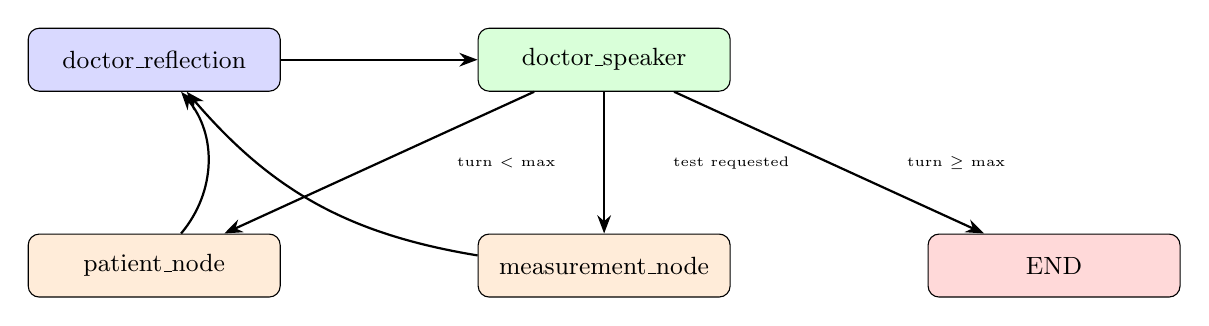
\begin{tikzpicture}[
    node distance=1.8cm and 2.5cm,
    every node/.style={draw, rounded corners, minimum width=3.2cm, minimum height=0.8cm, font=\small},
    arrow/.style={-Stealth, thick}
]
    \node[fill=blue!15]   (reflect)  {doctor\_reflection};
    \node[fill=green!15, right=of reflect]  (speak)    {doctor\_speaker};
    \node[fill=orange!15, below left=of speak]  (patient)   {patient\_node};
    \node[fill=orange!15, below=of speak]  (measure)  {measurement\_node};
    \node[fill=red!15,   below right=of speak] (end)   {END};

    \draw[arrow] (reflect) -- (speak);
    \draw[arrow] (speak) -- node[draw=none, right, font=\tiny]{turn \textless{} max} (patient);
    \draw[arrow] (speak) -- node[draw=none, right, font=\tiny]{test requested} (measure);
    \draw[arrow] (speak) -- node[draw=none, right, font=\tiny]{turn $\geq$ max} (end);
    \draw[arrow] (patient) to[bend right=40] (reflect);
    \draw[arrow] (measure) to[bend left=20] (reflect);
\end{tikzpicture}
\caption{LangGraph state machine for AgentClinic v2.1. The \texttt{doctor\_reflection} node performs latent metacognitive reasoning before each spoken turn.}
\end{figure}

\noindent\textbf{Key node responsibilities:}
\begin{itemize}
    \item \texttt{doctor\_reflection}: Silently updates the doctor's \textit{differential diagnosis list} without speaking to the patient. This makes latent LLM reasoning \textbf{observable and measurable} — a core thesis contribution.
    \item \texttt{doctor\_speaker}: Generates the actual spoken dialogue or final diagnosis.
    \item \texttt{patient\_node}: Patient LLM responds to the doctor's questions.
    \item \texttt{measurement\_node}: Measurement agent (lab test reader) returns test results.
\end{itemize}

\subsection{ClinicalState Schema}

The LangGraph state is typed via \texttt{ClinicalState (TypedDict)}:

\begin{lstlisting}[style=pystyle]
class ClinicalState(TypedDict):
    turn_count: int
    last_input_to_doctor: str
    last_doctor_message: str
    patient_response: str
    differential_diagnoses: List[str]
    differential_trajectory: Annotated[List, _list_concat]  # appends
    tests_ordered: Annotated[List, _list_concat]            # appends
    full_dialogue: List[dict]
    is_complete: bool
\end{lstlisting}

\noindent The use of \texttt{Annotated[List, \_list\_concat]} as a reducer enables automatic \textbf{trajectory accumulation} across graph steps — the full differential diagnosis history is available at the end of each case.

\subsection{Heterogeneous Multi-Engine Architecture}

A key innovation is the support for \textbf{different LLM backends per agent role}:

\begin{table}[H]
\centering
\caption{Heterogeneous engine assignment}
\begin{tabular}{@{}llll@{}}
\toprule
\textbf{Agent Role} & \textbf{Experiment E1} & \textbf{Experiment E2/E4/E5} & \textbf{Experiment E3} \\
\midrule
Doctor     & Mistral-7B-Instruct & JSL-MedMistral-7B & Llama-3.1-8B-Instruct \\
Patient    & Mistral-7B-Instruct & Mistral-7B-Instruct & Mistral-7B-Instruct \\
Measurement& Mistral-7B-Instruct & Mistral-7B-Instruct & Mistral-7B-Instruct \\
Moderator  & Mistral-7B-Instruct & Mistral-7B-Instruct & Mistral-7B-Instruct \\
\bottomrule
\end{tabular}
\end{table}

\noindent This design prevents \textbf{lexical leakage} — if all agents used the same weights, they might echo each other's phrasing rather than representing genuinely independent clinical perspectives.

\subsection{Local Inference with 4-bit Quantization}

The \texttt{LocalServerLLMWrapper} class loads HuggingFace models with optional \textbf{NF4 4-bit quantization} using \texttt{bitsandbytes}:

\begin{lstlisting}[style=pystyle]
bnb_config = BitsAndBytesConfig(
    load_in_4bit=True,
    bnb_4bit_quant_type="nf4",          # NormalFloat4 — lower error than int4
    bnb_4bit_use_double_quant=True,     # quantize the quantization constants
    bnb_4bit_compute_dtype=torch.float16
)
model = AutoModelForCausalLM.from_pretrained(
    model_id,
    quantization_config=bnb_config,
    device_map="auto",
    trust_remote_code=True,
    attn_implementation="eager"         # Flash Attention fallback
)
\end{lstlisting}

\noindent On the H100 (95.8 GB VRAM), Mistral-7B loads in roughly \textbf{5--6 GB} at 4-bit. During \textbf{E1}, quantization was disabled (\texttt{--no\_quantize}) to share the GPU under high contention from other lab users.

% ============================================================================
\section{Process-Oriented Evaluation Metrics}
% ============================================================================

The \texttt{ClinicalTrajectoryEvaluator} computes three metrics \textbf{inline} after each scenario, using the trajectory data accumulated in \texttt{ClinicalState}:

\subsection{Diagnostic Stability (DS)}

Measures how \textit{consistently} the doctor's differential diagnosis converges across turns. A higher value indicates less erratic hypothesis switching.

\[
DS = 1 - \frac{1}{T-1} \sum_{t=1}^{T-1} d_{\text{Jaccard}}(D_t, D_{t+1})
\]

where $D_t$ is the set of top-3 differential diagnoses at turn $t$, and $d_{\text{Jaccard}}$ is the Jaccard distance ($1 - \text{IoU}$). A DS of 1.0 means the differential never changed (maximum convergence); 0.0 means total instability.

\subsection{Test Rationality (TR)}

Binary measure: did the doctor order at least one medically relevant diagnostic test?
\[
TR = \mathbb{1}\left[\text{valid test name} \in \text{doctor's dialogue}\right] \in \{0, 1\}
\]

\subsection{Information Efficiency (IE)}

Measures how effectively the doctor uses each diagnostic turn:
\[
IE = \frac{N_{\text{unique diagnoses mentioned}}}{T_{\text{turns used}}}
\]
A value $> 1$ means the doctor explored more unique hypotheses than turns used (exploratory). A value $= 1$ is ideal convergence.

% ============================================================================
\section{Infrastructure \& Operations}
% ============================================================================

\subsection{GPU Watchdog Queue}

Because the H100 is shared across the lab, a custom \textbf{GPU Watchdog} (\texttt{gpu\_watchdog.sh}) was built to manage execution:

\begin{lstlisting}[style=bashstyle]
# Find a GPU with >= THRESHOLD MiB free VRAM
find_free_gpu() {
    local threshold=$1
    nvidia-smi --query-gpu=memory.free --format=csv,noheader,nounits \
    | awk -v t=$threshold 'NR>=1 && $1>=t {print NR-1, $1; exit}'
}
\end{lstlisting}

\noindent The watchdog supports three modes:
\begin{enumerate}
    \item \textbf{Single mode:} Wait for VRAM and run one command.\\
          \texttt{bash gpu\_watchdog.sh 15000 60 "bash run\_experiments.sh"}
    \item \textbf{Queue mode:} Continuously launch all experiments in \texttt{gpu\_queue.txt} as VRAM opens.\\
          \texttt{bash gpu\_watchdog.sh --queue gpu\_queue.txt 60}
    \item \textbf{Targeted mode:} Wait for VRAM and launch only one named experiment.\\
          \texttt{bash gpu\_watchdog.sh --run e2\_jsl\_med gpu\_queue.txt 60}
\end{enumerate}

\noindent Events are logged to \texttt{logs/watchdog\_events.txt} with timestamps and push notifications sent to the researcher's mobile via \textbf{ntfy.sh}.

\subsection{Mobile Notification System}

To allow hands-free monitoring, every major event triggers a push notification:

\begin{lstlisting}[style=bashstyle]
notify() { curl -s -d "$1" "ntfy.sh/agentclinic_dikshant_mtp" > /dev/null; }
\end{lstlisting}

Alerts are sent at:
\begin{itemize}
    \item Every 10 scenarios (progress checkpoint) from inside \texttt{agentic\_clinic\_v2.py}.
    \item On GPU launch from the watchdog (\texttt{gpu\_watchdog.sh}).
    \item On experiment block completion (\texttt{run\_experiments.sh}).
    \item On all-experiments-complete.
\end{itemize}

\subsection{Log Preservation}

To prevent log overwriting when re-running experiments, both \texttt{run\_experiments.sh} and \texttt{gpu\_watchdog.sh} use a \texttt{backup\_log()} function:

\begin{lstlisting}[style=bashstyle]
backup_log() {
    local logfile="$1"
    if [ -f "$logfile" ]; then
        local ts=$(date -r "$logfile" "+%Y%m%d_%H%M%S")
        mv "$logfile" "${logfile%.log}_${ts}.log"
    fi
}
\end{lstlisting}

\noindent Old logs are renamed with a timestamp suffix (e.g., \texttt{e1\_baseline\_20260416\_121629.log}).

\subsection{Pipeline \& Python Buffering Note}

During E1, a buffering issue was observed: the log file (\texttt{e1\_baseline.log}) appeared to stop updating at Scenario 66 while the terminal showed Scenario 99. This is a standard Linux \textbf{pipe buffering} behaviour — when Python stdout is piped into \texttt{tee}, it switches to 8KB block buffering instead of line buffering. \textbf{No data was lost}; the buffer flushed automatically when the block filled. For future runs, add \texttt{-u} (unbuffered) to the Python invocation to eliminate the appearance of lag:
\begin{lstlisting}[style=bashstyle]
python -u "${SCRIPT}" ... 2>&1 | tee "${LOG_DIR}/e1_baseline.log"
\end{lstlisting}

% ============================================================================
\section{Experiment Matrix}
% ============================================================================

\begin{table}[H]
\centering
\caption{Full experiment matrix — 107 MedQA scenarios, 10 turns per scenario}
\begin{tabular}{@{}lllllll@{}}
\toprule
\textbf{ID} & \textbf{Name} & \textbf{Doctor Model} & \textbf{Patient Model} & \textbf{Bias} & \textbf{Quant?} & \textbf{Status} \\
\midrule
E0 & Smoke Test & Mistral-7B & Mistral-7B & None & No  & \textcolor{successpink}{\checkmark Complete} \\
E1 & Baseline   & Mistral-7B & Mistral-7B & None & No  & \textcolor{successpink}{\checkmark Complete} \\
E2 & JSL-Med Doctor & JSL-MedMistral-7B & Mistral-7B & None & Yes & In Progress \\
E3 & Llama Doctor   & Llama-3.1-8B      & Mistral-7B & None & Yes & Pending \\
E4 & Recency Bias   & JSL-MedMistral-7B & Mistral-7B & Recency & Yes & Pending \\
E5 & Confirm. Bias  & JSL-MedMistral-7B & Mistral-7B & Confirmation & Yes & Pending \\
\bottomrule
\end{tabular}
\end{table}

\noindent\textbf{Hypothesis:} JSL-MedMistral-7B (E2) will outperform Mistral-7B (E1) due to medical domain fine-tuning. Cognitive biases (E4, E5) will \textit{decrease} accuracy and \textit{increase} diagnostic instability relative to E2.

% ============================================================================
\section{Results — Experiment E1 (Baseline)}
% ============================================================================

\subsection{Setup}
\begin{itemize}
    \item \textbf{Dataset:} MedQA (USMLE-style multiple choice, converted to open-ended format)
    \item \textbf{Doctor Model:} \texttt{mistralai/Mistral-7B-Instruct-v0.2} (all roles, homogeneous)
    \item \textbf{Scenarios:} 107 (full MedQA subset)
    \item \textbf{Max Turns:} 10 per scenario
    \item \textbf{Quantization:} Disabled (fp16) due to GPU contention
    \item \textbf{Duration:} $\approx$3.7 hours on H100 NVL
\end{itemize}

\subsection{Outcome Accuracy}

\begin{table}[H]
\centering
\caption{E1 Baseline — Final diagnostic accuracy}
\begin{tabular}{@{}lrr@{}}
\toprule
\textbf{Metric}          & \textbf{Value} & \textbf{Note} \\
\midrule
Total Scenarios          & 107   & Full MedQA subset \\
Correct Diagnoses        & 36    & Semantic match via moderator \\
\textbf{Accuracy}        & \textbf{33.6\%} & Mistral-7B homogeneous baseline \\
\bottomrule
\end{tabular}
\end{table}

\noindent\textbf{Interpretation:} A 33.6\% accuracy on USMLE-format questions is consistent with findings from the original AgentClinic paper, where GPT-3.5 (a much stronger model) achieved $\approx$37--42\%. Given that Mistral-7B is a 7B parameter model accessed locally, this establishes a \textbf{realistic lower-bound baseline} for the follow-up heterogeneous experiments.

\subsection{Process Metrics}

\begin{table}[H]
\centering
\caption{E1 Baseline — Averaged process-oriented metrics ($n=107$ scenarios)}
\begin{tabular}{@{}lrrr@{}}
\toprule
\textbf{Metric} & \textbf{Mean} & \textbf{Interpretation} & \textbf{Range} \\
\midrule
Diagnostic Stability (DS) & $\approx$ 0.56 & Moderate convergence & {[0, 1]} \\
Test Rationality (TR)     & $\approx$ 0.63 & 63\% of cases ordered relevant tests & \{0, 1\} \\
Information Efficiency (IE) & $\approx$ 1.13 & Slightly exploratory & (0, $\infty$) \\
\bottomrule
\end{tabular}
\end{table}

\noindent\textbf{Key observations:}
\begin{itemize}
    \item A DS of 0.56 indicates that Mistral-7B's differential diagnosis \textit{shifts significantly} across turns — it does not commit early to a strong hypothesis. This is expected from a general-purpose model without clinical grounding.
    \item TR of 63\% shows the model attempts diagnostic testing in the majority of cases, a healthy clinical behaviour.
    \item IE $> 1$ is expected at 10 turns; most cases had 2--4 unique diagnoses explored across 10 turns of dialogue.
\end{itemize}

% ============================================================================
\section{Key Technical Contributions vs. Phase 1}
% ============================================================================

\begin{table}[H]
\centering
\caption{Comparison of Phase 1 legacy vs. Phase 2 (v2.1) implementation}
\begin{tabular}{@{}p{5cm}p{4.5cm}p{4.5cm}@{}}
\toprule
\textbf{Feature} & \textbf{Phase 1 (Legacy)} & \textbf{Phase 2 (v2.1)} \\
\midrule
State Management          & Ad hoc while-loop        & LangGraph DCG (deterministic) \\
Local Model Inference     & None (API only)          & HuggingFace + 4-bit NF4 Quant \\
Heterogeneous Architecture & No (single model)       & Yes (doctor $\neq$ patient) \\
Trajectory Logging        & None                     & Full differential trajectory \\
Metrics Computation       & Post-hoc script          & Inline per-scenario \\
GPU Resource Management   & None                     & Watchdog queue (3 modes) \\
Bias Implementation       & Prompt only              & Prompt + structured injection \\
Mobile Notifications      & None                     & ntfy.sh integration \\
Log Preservation          & Overwrites               & Timestamped backups \\
Smoke Test                & None                     & E0 (3 scenarios, 5 turns) \\
\bottomrule
\end{tabular}
\end{table}

% ============================================================================
\section{Repository Structure}
% ============================================================================

\begin{lstlisting}[style=bashstyle]
AgentClinic/
  agentic_clinic_v2.py       # Core framework (LangGraph DCG, all agents)
  run_experiments.sh         # Full E0-E5 experiment launcher
  gpu_watchdog.sh            # GPU queue manager (3 modes)
  gpu_queue.txt              # Experiment queue with VRAM requirements
  requirements.txt           # Python dependencies
  implementation_report.tex  # Earlier LaTeX architecture report
  thesis_progress_report.tex # This document
  results/
    results_Mistral-7B_*.jsonl  # Per-scenario JSONL from E1
  logs/
    e0_smoke_test.log        # E0 output
    e1_baseline.log          # E1 complete output (107 scenarios)
    e2_jsl_med.log           # E2 (in progress)
    watchdog_events.txt      # GPU launch events + timestamps
\end{lstlisting}

% ============================================================================
\section{Current Status \& Next Steps}
% ============================================================================

\subsection{Current Status (as of April 17, 2026)}

\begin{itemize}
    \item[\textcolor{successpink}{\checkmark}] \textbf{E0 Smoke Test} — Complete. Pipeline validated.
    \item[\textcolor{successpink}{\checkmark}] \textbf{E1 Baseline} — Complete. 107/107 scenarios. Accuracy: 33.6\%.
    \item[$\rightarrow$]                        \textbf{E2 JSL-Med Doctor} — In progress (running via watchdog).
    \item[$\circ$]                              \textbf{E3 Llama-3.1-8B Doctor} — Pending.
    \item[$\circ$]                              \textbf{E4 Recency Bias} — Pending.
    \item[$\circ$]                              \textbf{E5 Confirmation Bias} — Pending.
\end{itemize}

\subsection{Expected Results When All Experiments Complete}

\begin{table}[H]
\centering
\caption{Anticipated results table (to be filled in)}
\label{tab:results_full}
\begin{tabular}{@{}lllllll@{}}
\toprule
\textbf{Exp.} & \textbf{Doctor} & \textbf{Bias} & \textbf{Acc.} & \textbf{DS} & \textbf{TR} & \textbf{IE} \\
\midrule
E1 & Mistral-7B     & None         & 33.6\% & $\sim$0.56 & $\sim$0.63 & $\sim$1.13 \\
E2 & JSL-MedMistral & None         & TBD    & TBD & TBD & TBD \\
E3 & Llama-3.1-8B   & None         & TBD    & TBD & TBD & TBD \\
E4 & JSL-MedMistral & Recency      & TBD    & TBD & TBD & TBD \\
E5 & JSL-MedMistral & Confirmation & TBD    & TBD & TBD & TBD \\
\bottomrule
\end{tabular}
\end{table}

\subsection{Immediate Next Steps}

\begin{enumerate}
    \item \textbf{Monitor E2:} \texttt{tail -f logs/e2\_jsl\_med.log} or check ntfy app.
    \item \textbf{After E2 completes:} Launch E3 via the watchdog queue.
    \item \textbf{Analysis Script:} Once all JSONL files are present in \texttt{results/}, run a Jupyter analysis to:
    \begin{itemize}
        \item Aggregate per-experiment means and confidence intervals.
        \item Generate Alluvial diagrams of bias effect on diagnostic trajectory.
        \item Generate radar charts of DS/TR/IE per experiment.
    \end{itemize}
    \item \textbf{Fix buffering:} Add \texttt{-u} to Python calls in \texttt{run\_experiments.sh}.
    \item \textbf{Fix E1 syntax issue:} The \texttt{backup\_log} line is misplaced (on the \texttt{python} continuation line) for E1--E5. This needs correction before next run.
    \item \textbf{Thesis writing:} Use E1 results as the baseline section; update Table \ref{tab:results_full} when all experiments complete.
\end{enumerate}

% ============================================================================
\section{Known Issues \& Mitigations}
% ============================================================================

\begin{table}[H]
\centering
\caption{Known issues and their mitigations}
\begin{tabular}{@{}p{5cm}p{4cm}p{4.5cm}@{}}
\toprule
\textbf{Issue} & \textbf{Cause} & \textbf{Mitigation} \\
\midrule
Log appears to stop updating mid-run & Pipe block buffering (8KB chunks) & Add \texttt{python -u}; no data is lost \\
OOM on H100 during loading & VRAM fragmentation from other users & Raise watchdog threshold; use \texttt{expandable\_segments=True} \\
\texttt{backup\_log} on continuation line in E1-E5 & \texttt{sed} insertion at wrong line in script & Fix before next run (see Section 8.2) \\
E2 launched twice (once via queue, once manually) & Duplicate watchdog processes & Use only one watchdog mode per session \\
\texttt{tee} overwrites log on re-run & Default \texttt{tee} behavior & \texttt{backup\_log()} now prepended to each block \\
\bottomrule
\end{tabular}
\end{table}

% ============================================================================
\section{For Future AI Agents: Quick Resume Guide}
% ============================================================================

\begin{tcolorbox}[colback=noteblue, colframe=iitblue, title=\textbf{If you are resuming this project as an AI agent, read this first}]

\textbf{Environment:}
\begin{itemize}
    \item Python virtual env: \texttt{\textasciitilde/.venv} or \texttt{test\_venv/}. Activate with: \texttt{source test\_venv/bin/activate}
    \item Working dir: \texttt{\textasciitilde/mtp-agentclinic/AgentClinic/}
    \item GPU: Single NVIDIA H100 NVL (95.8~GB), shared with other lab users.
\end{itemize}

\textbf{Key files to read first:}
\begin{enumerate}
    \item \texttt{agentic\_clinic\_v2.py} — core logic (LangGraph, agents, metrics, quantization)
    \item \texttt{run\_experiments.sh} — experiment configuration (models, VRAM, bias settings)
    \item \texttt{gpu\_watchdog.sh} — GPU queue manager
    \item \texttt{results/*.jsonl} — one line per scenario with all metrics
\end{enumerate}

\textbf{Check experiment status:}
\begin{lstlisting}[style=bashstyle]
tail -f logs/e2_jsl_med.log           # Monitor E2 progress
grep "Running Accuracy" logs/e1_baseline.log | tail -3  # E1 final acc
ls -la results/*.jsonl                 # See which results exist
\end{lstlisting}

\textbf{Known bug to fix before next run:} In \texttt{run\_experiments.sh}, lines 78, 100, 122, 144, 166 have \texttt{backup\_log} placed \textit{after} the \texttt{python "\$\{SCRIPT\}"} backslash continuation, which will cause a parse error. The correct form should be:
\begin{lstlisting}[style=bashstyle]
backup_log "${LOG_DIR}/e1_baseline.log"   # BEFORE the python call
python "${SCRIPT}" \
    --doctor_llm ...
\end{lstlisting}

\textbf{Mobile notifications:} Topic \texttt{agentclinic\_dikshant\_mtp} on ntfy.sh. Test with:
\texttt{curl -d "test" ntfy.sh/agentclinic\_dikshant\_mtp}
\end{tcolorbox}

% ============================================================================
\appendix
\section{Model Information}
% ============================================================================

\begin{table}[H]
\centering
\caption{HuggingFace models used in this study}
\begin{tabular}{@{}lllll@{}}
\toprule
\textbf{Model} & \textbf{Params} & \textbf{Training} & \textbf{HF ID} & \textbf{VRAM (4-bit)} \\
\midrule
Mistral-7B-Instruct-v0.2 & 7B & General instruct & mistralai/Mistral-7B-Instruct-v0.2 & $\sim$5 GB \\
JSL-MedMistral-7B-v2.2   & 7B & Medical (JohnSnowLabs) & johnsnowlabs/JSL-MedMistral-7B-v2.2 & $\sim$5 GB \\
Llama-3.1-8B-Instruct    & 8B & General instruct & meta-llama/Llama-3.1-8B-Instruct & $\sim$6 GB \\
\bottomrule
\end{tabular}
\end{table}

\section{Key Python Dependencies}

\begin{lstlisting}[style=bashstyle]
torch>=2.0.0
transformers>=4.40.0
accelerate>=0.30.0
bitsandbytes>=0.43.0        # 4-bit NF4 quantization
langgraph>=0.0.40            # State machine orchestration
langchain-core>=0.2.0
openai==0.28.0               # Legacy API (for Replicate/OpenAI)
scipy>=1.10.0                # Statistical analysis (post-processing)
pandas>=2.0.0
matplotlib>=3.7.0
seaborn>=0.12.0
\end{lstlisting}

\vspace{2em}
\hrule
\vspace{0.5em}
\noindent\textit{Last updated: April 17, 2026. Generated by the AI coding assistant as a reference document for Dikshant Sharma's M.Tech thesis, IIT Kharagpur.}

\end{document}
